\documentclass[12pt]{ctexart}

\usepackage{graphicx}
\usepackage[hmargin=1.1in,vmargin=1in]{geometry}
\usepackage{indentfirst}
\usepackage{multirow}
\usepackage{makecell}
\usepackage{gbt7714}
\usepackage[defaultmono,scale=0.85]{droidsansmono}
\usepackage[colorlinks=true]{hyperref}

\bibliographystyle{gbt7714-numerical}

\fontsize{14pt}{1.0}

\newlength{\blanklength}
\setlength{\blanklength}{40ex}

\providecommand{\thetitle}{光线追踪}
\providecommand{\theauthor}{Sparky\_14145}
\providecommand{\thestudentID}{71XXXXXX}
\providecommand{\theemail}{Sparky\_14145@outlook.com}
\providecommand{\theinstitution}{College of Software Engineering}

% \input{personal_info/info.tex}

\providecommand{\blankToFill}[1]{
    \parbox[t][3ex]{\blanklength}{
        \makebox[\blanklength]{#1}\\[0pt]
        \rule[2ex]{\blanklength}{0.1ex}
    }
}

\providecommand{\makecover}{\begin{titlepage}
    \noindent
    {东南大学} \\[2pt]
    {\Large \bfseries 课程报告}

    \vspace*{20pt}
    \begin{center}
    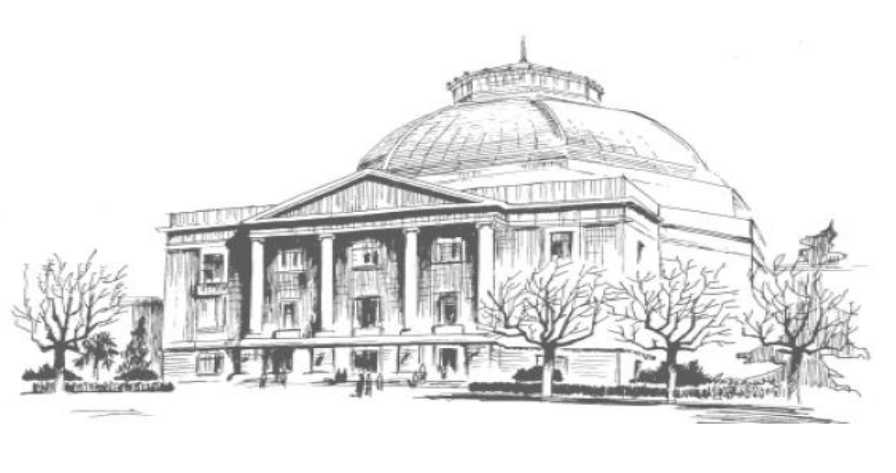
\includegraphics[width=0.8\textwidth]{pics/cover.png} \\
        \textsc{\Huge 计算机图形学} \\[2pt]
        \textsc{\huge 课程报告}

        \vspace*{10pt}
        \begin{tabular}[c]{rc}
            题目        & \blankToFill{\thetitle} \\
            日期        & \blankToFill{\today} \\
            姓名        & \blankToFill{\theauthor\footnotemark} \\
            学号        & \blankToFill{\thestudentID} \\
            学院        & \blankToFill{\theinstitution} 
        \end{tabular}
        \rmfamily
    \end{center}

    \vspace*{0pt}
    \footnotetext{\theemail}
\end{titlepage}}

\begin{document}
    \makecover

    \section{背景}

    在光线追踪以前,计算机渲染三维图形都是通过将三维空间利用坐标变换的方法投影到二维屏幕上的。这种做法比较简单,并且很多时候也``够用''了,但是在对图形渲染要求更加精细的地方,比如说在对能够反光的物体表面进行渲染时,用坐标变换就不能很好地反应光线的反射效果等了。为此,计算机科学家们尝试模拟真实世界中光线沿直线传播、在表面进行反射等特性,提出了光线追踪的思想,并基于这种思想提出了多种光线追踪算法,旨在得到对于建模完成的物体与给定的光照条件下,得到更好的渲染效果以及更好的性能。

    \section{概述}

    如前所述,光线追踪是一大类渲染算法的统称。一般来说,光线追踪算法基于以下(实际上并完全不正确的)假设:

    \begin{enumerate}
        \item 光线沿直线传播;
        \item 相交的光线彼此之间互不影响;
        \item 光线从光源发出进入观察者的眼睛;
        \item 光路可逆(允许只计算通过视平面处有限个像素并进入观察者眼睛的光线来减少运算量)。
    \end{enumerate}
    
    相比于坐标变换,光线追踪算法渲染出的图形质量往往要高得多,而代价是渲染图形所需要的算力也高了不少,故尽管光线追踪算法事实上上个世纪便已经开始研究,直到最近几年,随着 GPU 硬件的不断改进,实时的、家用的游戏内光线追踪才逐渐得到普及。

    \section{几个光线追踪算法}

    \subsection{Ray Casting}

    最为简单的光线追踪算法,于 1968 年提出。

    基本思想是从观察者的眼睛向各个像素``射出''一道道``视线'',计算这些``视线''与物体表面的第一个交点以及反射情况,然后再与光源到反射点处的向量进行相关运算,确定各个光源对该点该方向上的亮度以及颜色的贡献,最后再叠加这些影响得到最终的渲染效果。

    如果不考虑物体间的相互作用,显然这个算法已经能够渲染出较高质量的图片了。不过这个算法的问题就是,无法正确处理多个物体(或者同一个物体不同表面)之间光线反射造成的影响。

    \subsection{Recursive Ray Tracing}

    本质上也是一种 Ray Casting,但是在计算出``视线''与物体表面的第一个交点以后不是停止追踪光线,而是分析出光线的反射、折射方向,并沿着这些方向继续递归地进行光线追踪,并且每遇到一个交点之后都会计算一次与光源的``照射关系'',在计算这些与光源的``照射关系''时,光线与其他物体的遮挡关系也会被考虑,从而模拟出阴影效果。

    这种算法是 Ray Casting 的一个改进,事实上也确实大幅度改进了渲染效果。但是存在一些问题:需要追踪的光线数量会随着递归追踪的次数呈指数增长,并且有的时候,``视线''会无限制地反射下去。幸运的是,一般来说,光线在反射与折射时强度会衰减,而多次反射与折射后这些光线的实际作用就可以忽略不计了。因此在实际实现中,这个算法往往会限制递归的最大次数,以改进性能。

\end{document}